\section{Background Estimation}
\label{sec:analysis:background}





This analysis has three main sources of backgrounds:

\begin{itemize}
    \item vector boson plus jets
    \item multijet QCD
    \item diboson production
\end{itemize}

Vector boson (W or Z) production is the most prominent source of backgrounds overall.  These processes are well modelled and the simulation is found to be sufficient for the precision of modelling we require.  Diboson production is similarily well modelled, but is far less significant.  

It is worth pointing out that normalization of the W+jet, WW, and WZ production will all be sensitive to variations of the W decay branching fractions.  In general the yield from these processes are very small compared to \ttbar and tW production.  It is also the case that we assume fairly conservative uncertainties on the normalization of these processes ($\geq 5\%$) such that there should not be any sensitivity to the effect of the variation of the branching fractions.  For the case of the shape analysis, the W + jets sample is treated as a signal sample and is decomposed based on the decay modes of the W boson.  

The multijet QCD background affects the $e\tau$, $e$ + jets, $\mu\tau$, and $\mu$ + jets channels.  The number of generated events for this process is found to be insufficient for accurately modelling the event yields and shapes for this process so data-driven methods are employed.

The breakdown of predicted backgrounds are shown in tables~\ref{tab:yields} and \ref{tab:yields_ltau}.   


In several of the selected channels there is a non-negligible contamination from non-prompt production of leptons, in particular, the channels targetting semi-leptonic \ttbar decays and decays with hadronic taus in the final state.  One production process that gives rise to these events for which there is insufficient MC events is multiplepton QCD.  These events tend to affect selections where there is only one electron or muon.  This background is estimated using two different methods: for the semileptonic \ttbar selections, an estimate based on the fake rate method is used; for the hadronic $\tau$ final states, a sideband selected by inverting the dilepton charge requirement is used for the estimate.



\subsection{Fake rate method}

A commonly used method for estimating backgrounds from misidentified prompt lepton production can be summarized as follows:

\begin{enumerate}
    \item construct a control region that is enhanced in the production of leptons from non-prompt sources,
    
    \item measure the ratio, the ``fake rate", of the number of leptons passing a loose selection criteria to the number passing a tighter selection, i.e., the number of muons passing the analysis isolation requirement to those that pass with no isolation requirement,
    
        \begin{equation}
            f = \frac{N_{\rm pass\ iso}}{N_{\rm no iso}}
        \end{equation}

    \item apply a weight based on the fake rate ($w = f/(1-f)$) to events in the signal region where the leptons are required to pass the loose requirement but fail the tight requirement.
\end{enumerate}

The control region that is used for the fake rate measurement is selected to be enhanced in Z plus jet production.  Specifically, it is required that:

\begin{itemize}
    \item there are at least two muons or electrons passing the full analysis requirements,
    \item the two leptons must have opposite signs,
    \item $|M_{\ell\ell} - M_{Z}| < 15~\GeV$,
    \item the dilepton pair that has mass closest to the Z boson is selected
    \item one additional lepton (muon or electron) passing all
    identification requirements except the isolation requirement
\end{itemize}

The additional lepton is assumed to originate from an hadronic jet that is produced in association with the Z boson, but can frequently arise due to a prompt lepton produced from a diboson process such as WZ or ZZ production.  This is accounted for by subtracting off the estimate of these processes from simulation from the data in the fake rate control region.  Figures~\ref{fig:lepton_fr} show the measured \pt distributions of the electron and muon candidates and the resulting fake rates and the values for each of the \pt bins are shown in table~\ref{tab:lepton_fr}.


\begin{figure}
    \centering
    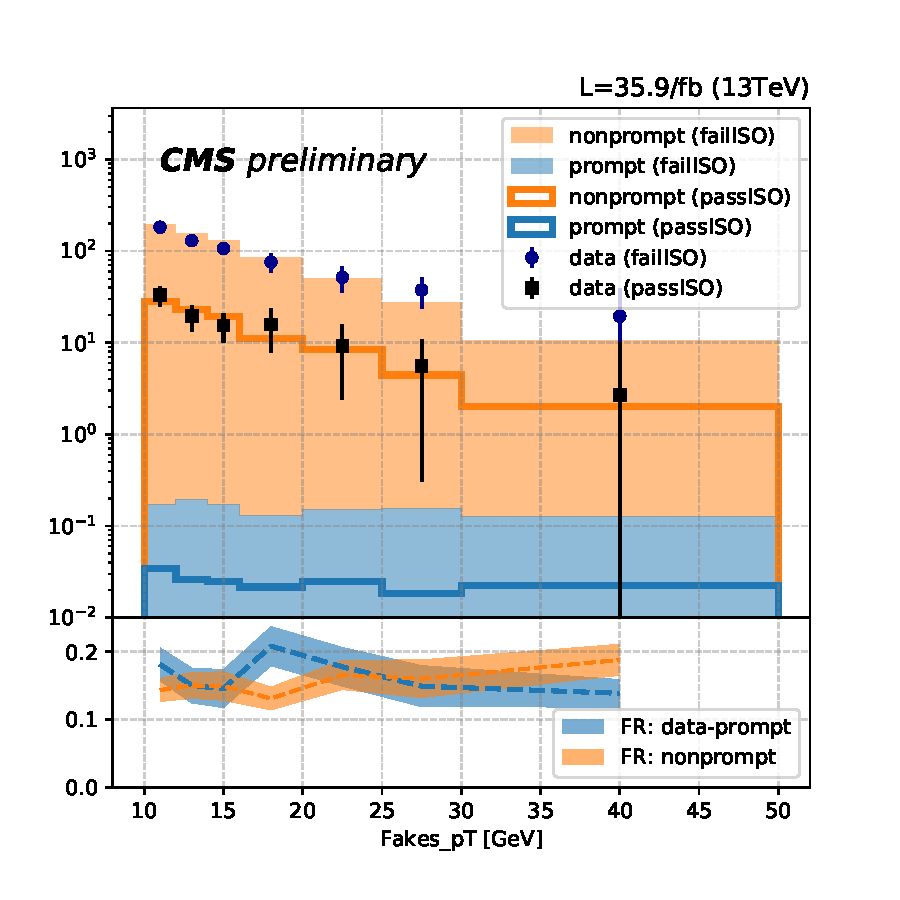
\includegraphics[width=0.45\textwidth]{chapters/Analysis/sectionBackground/figures/e_fakerate}
    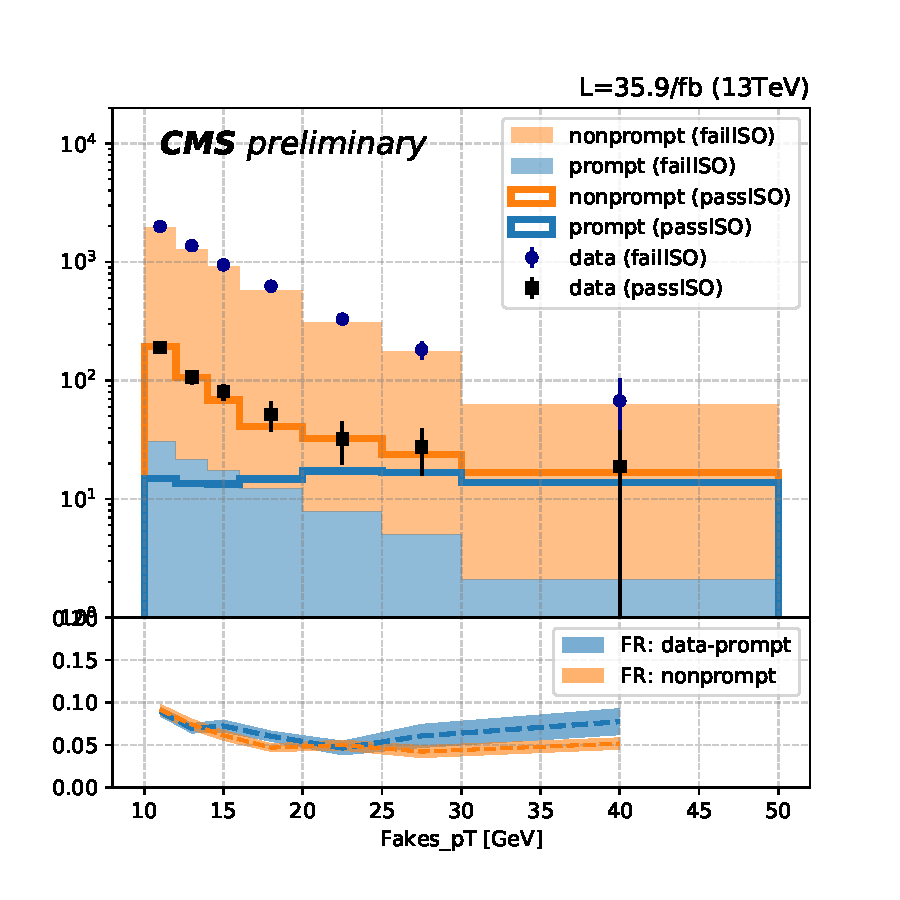
\includegraphics[width=0.45\textwidth]{chapters/Analysis/sectionBackground/figures/mu_fakerate}
    \caption{\pt distributions for the electron (left) and muon (right) fake candidates in the Z enriched control region.  The bottom panels show the measured fake rates}
    \label{fig:lepton_fr}
\end{figure}


\begin{table}[ht]
	\setlength{\tabcolsep}{1em}
    \renewcommand{\arraystretch}{1.5}
  	\centering
  	\caption{Fake rate for muon candidate (left) and electron candidate (right) }
  	\begin{tabular}{l|ll|ll}
  	\hline
  	        & \multicolumn{2}{c|}{Z+mu}          & \multicolumn{2}{c}{Z+e}           \\
	\hline
	pT bins & Data-VV            & DY+tt+tW         & Data-VV            & DY+tt+tW         \\
	\hline
    10-12   & 0.090$\pm$0.003    & 0.097$\pm$0.004  & 0.055$\pm$0.005    & 0.046$\pm$0.006  \\
    12-14   & 0.075$\pm$0.003    & 0.075$\pm$0.003  & 0.060$\pm$0.006    & 0.076$\pm$0.009  \\
    14-16   & 0.072$\pm$0.004    & 0.070$\pm$0.004  & 0.070$\pm$0.008    & 0.066$\pm$0.009  \\
    16-18   & 0.064$\pm$0.004    & 0.059$\pm$0.004  & 0.057$\pm$0.008    & 0.055$\pm$0.009  \\
    18-20   & 0.064$\pm$0.005    & 0.060$\pm$0.004  & 0.065$\pm$0.010    & 0.102$\pm$0.017  \\
    20-25   & 0.059$\pm$0.005    & 0.060$\pm$0.003  & 0.084$\pm$0.010    & 0.097$\pm$0.010  \\
    25-40   & 0.096$\pm$0.007    & 0.067$\pm$0.003  & 0.125$\pm$0.013    & 0.108$\pm$0.012  \\
    40-60   & 0.167$\pm$0.021    & 0.135$\pm$0.008  & 0.250$\pm$0.040    & 0.147$\pm$0.023  \\
    \hline
    \end{tabular}
    
    \label{tab:lepton_fr}
\end{table}




The fake rate that is applied to the data in the isolation sideband of the signal region is the one derived from data.  The systematic uncertainty on this background is conservatively treated as being 30\% for both electron and muon fakes.  

\FloatBarrier



\subsection{Same-sign estimate}

This estimation relies on the dearth of standard model processes that can give rise to same-sign lepton pairs.  Because of this it is expected that most events with same-sign lepton pairs are the result of at least on of the leptons not being the result of a prompt bosonic decay, but are produced by a hadronic jet.  It is further assumed that this process will give rise to misidentifying hadronic jets as leptons in near equal measure between the same sign and opposite sign selections.  This is verified by deriving a scale factor in an isolation inverted region.

The process of deriving the estimate is simple enough: all the same selection requirements that are applied in the nominal analysis selection are applied to the side-band region with the exception of the opposite sign requirement, which is inverted.  The same is done for all of the relevant MC samples in order to determine what component of the same-sign data sample will already be estimated by the MC.  Finally, a correction factor is applied to account for any difference in the probability of the QCD giving rise to opposite sign and same sign final states.

To verify the method, a control region enriched in $\PZ\to\tau\tau$ is examined for the $\mu\tau$ and $e\tau$ final states.  A comparison of data and simulation in both the same sign and opposite sign regions are shown in figure~\ref{fig:ltau_fakes}.

\begin{figure}
    \centering
    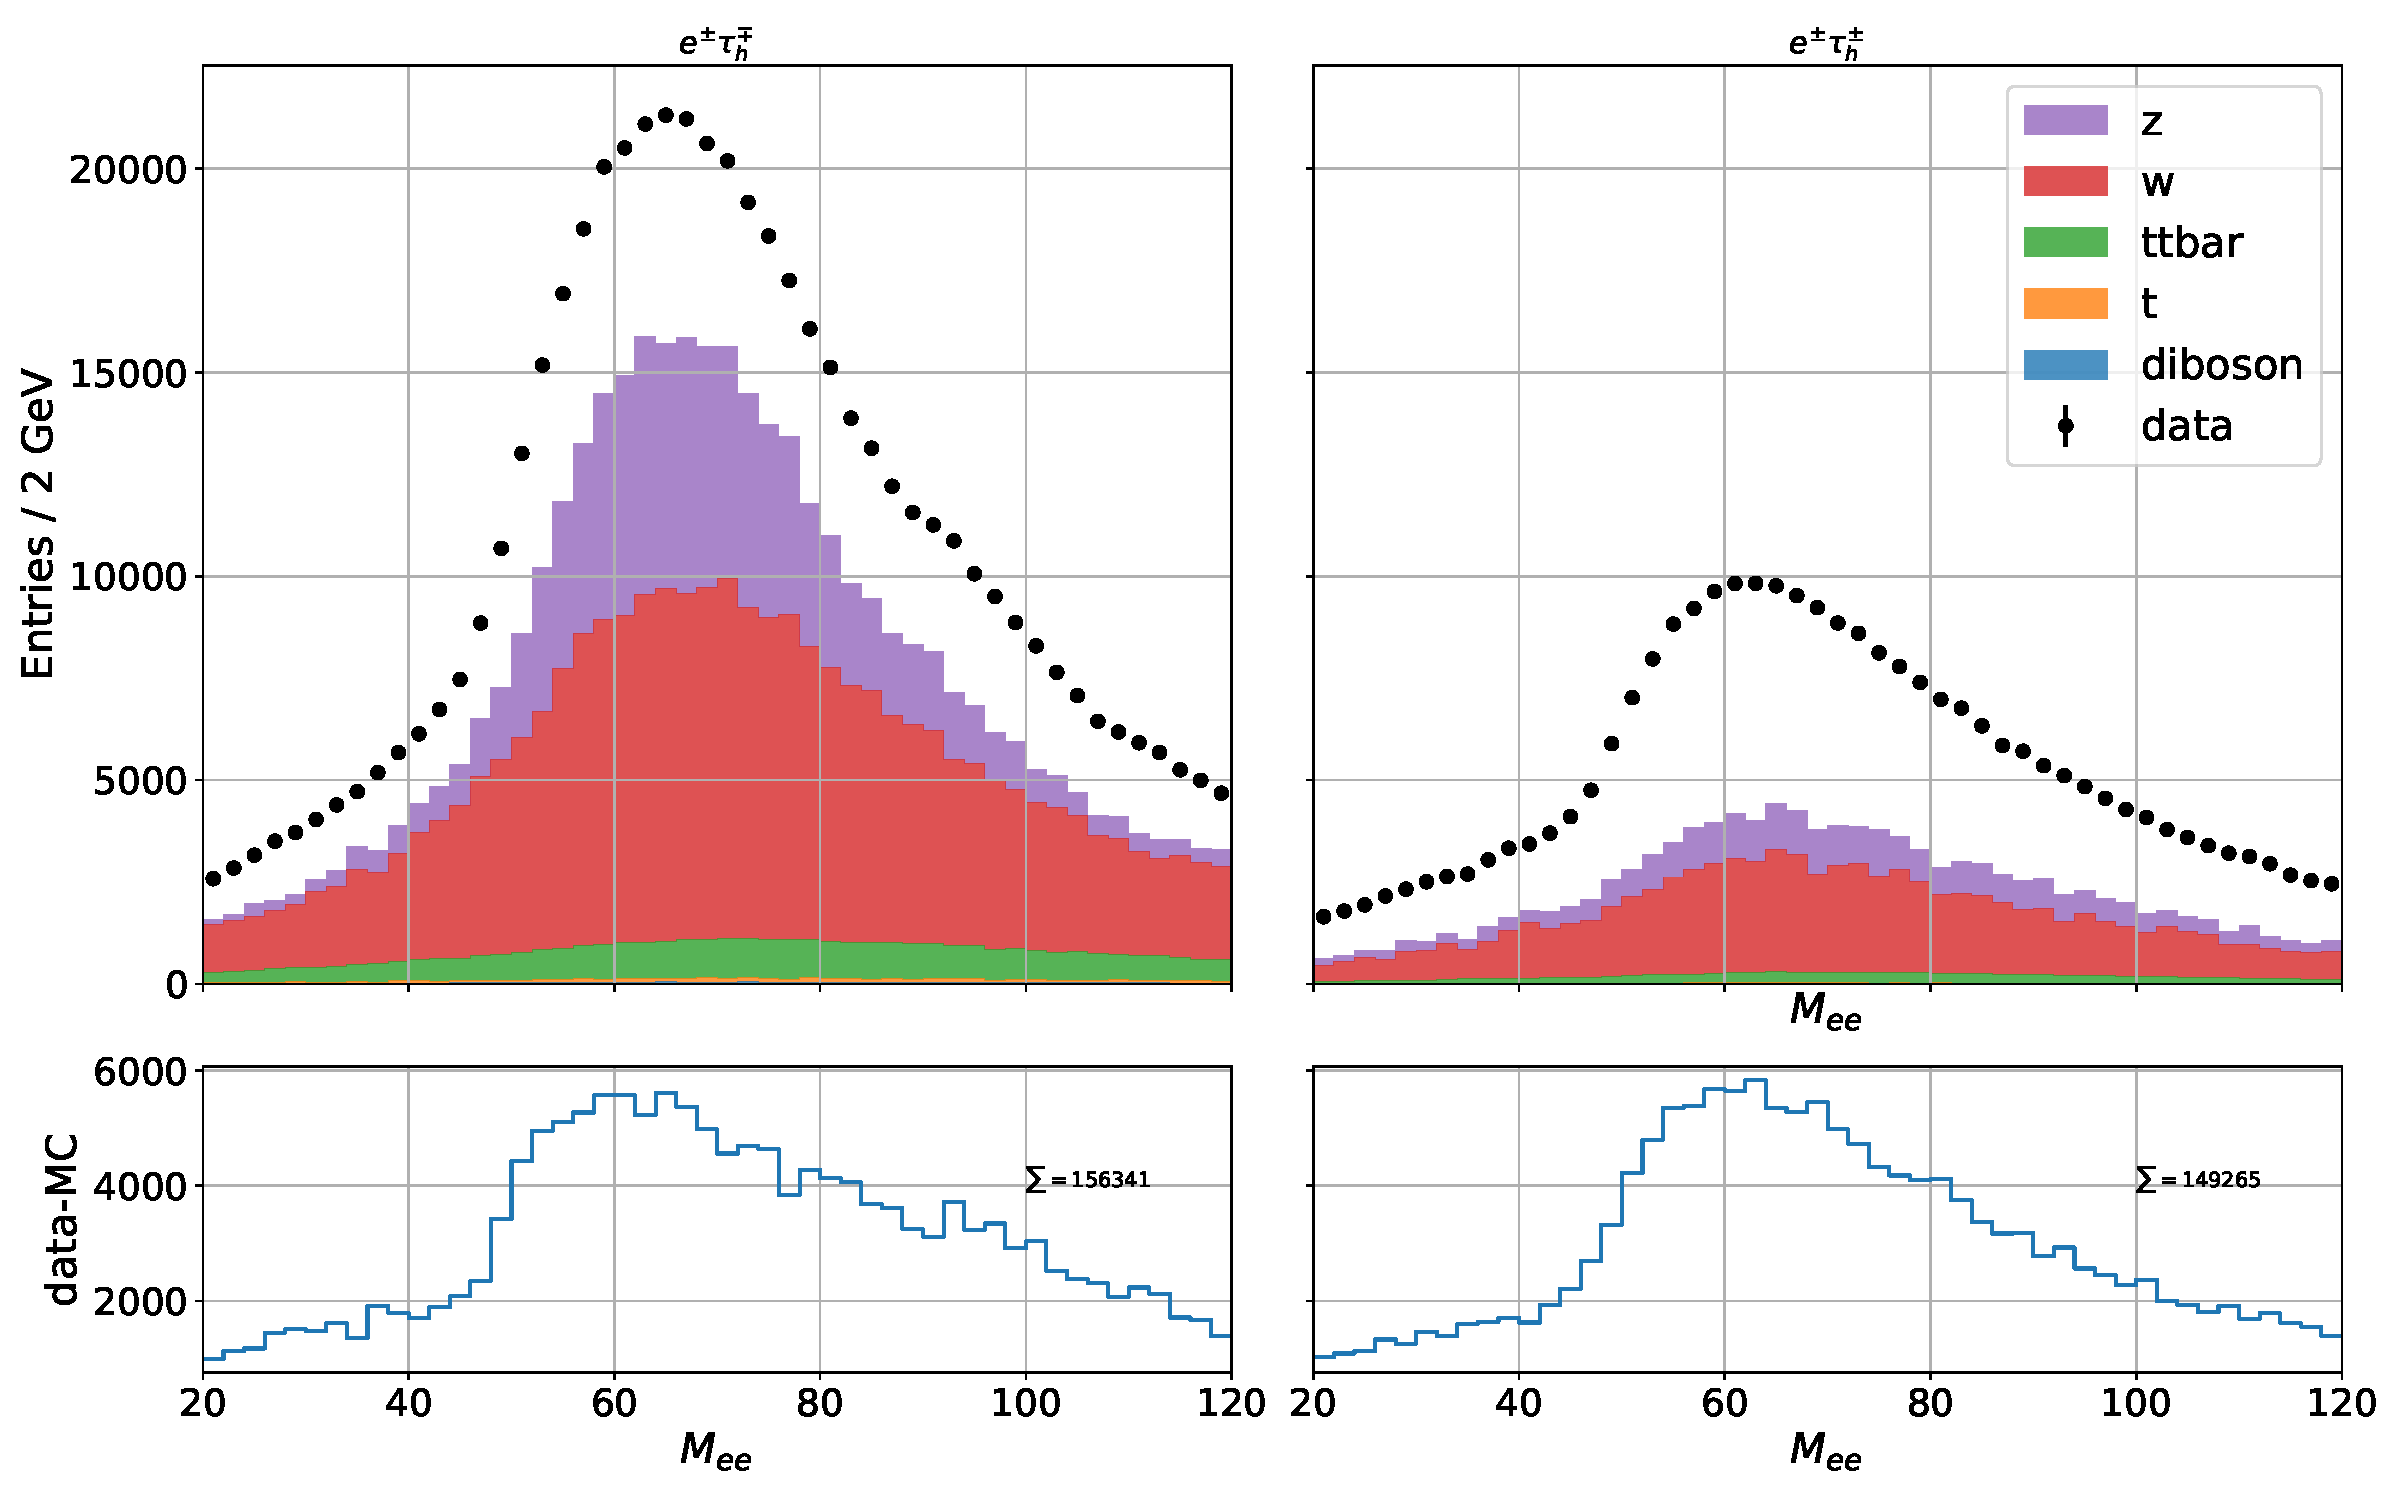
\includegraphics[width=0.9\textwidth]{chapters/Analysis/sectionBackground/figures/etau_cr.pdf}
    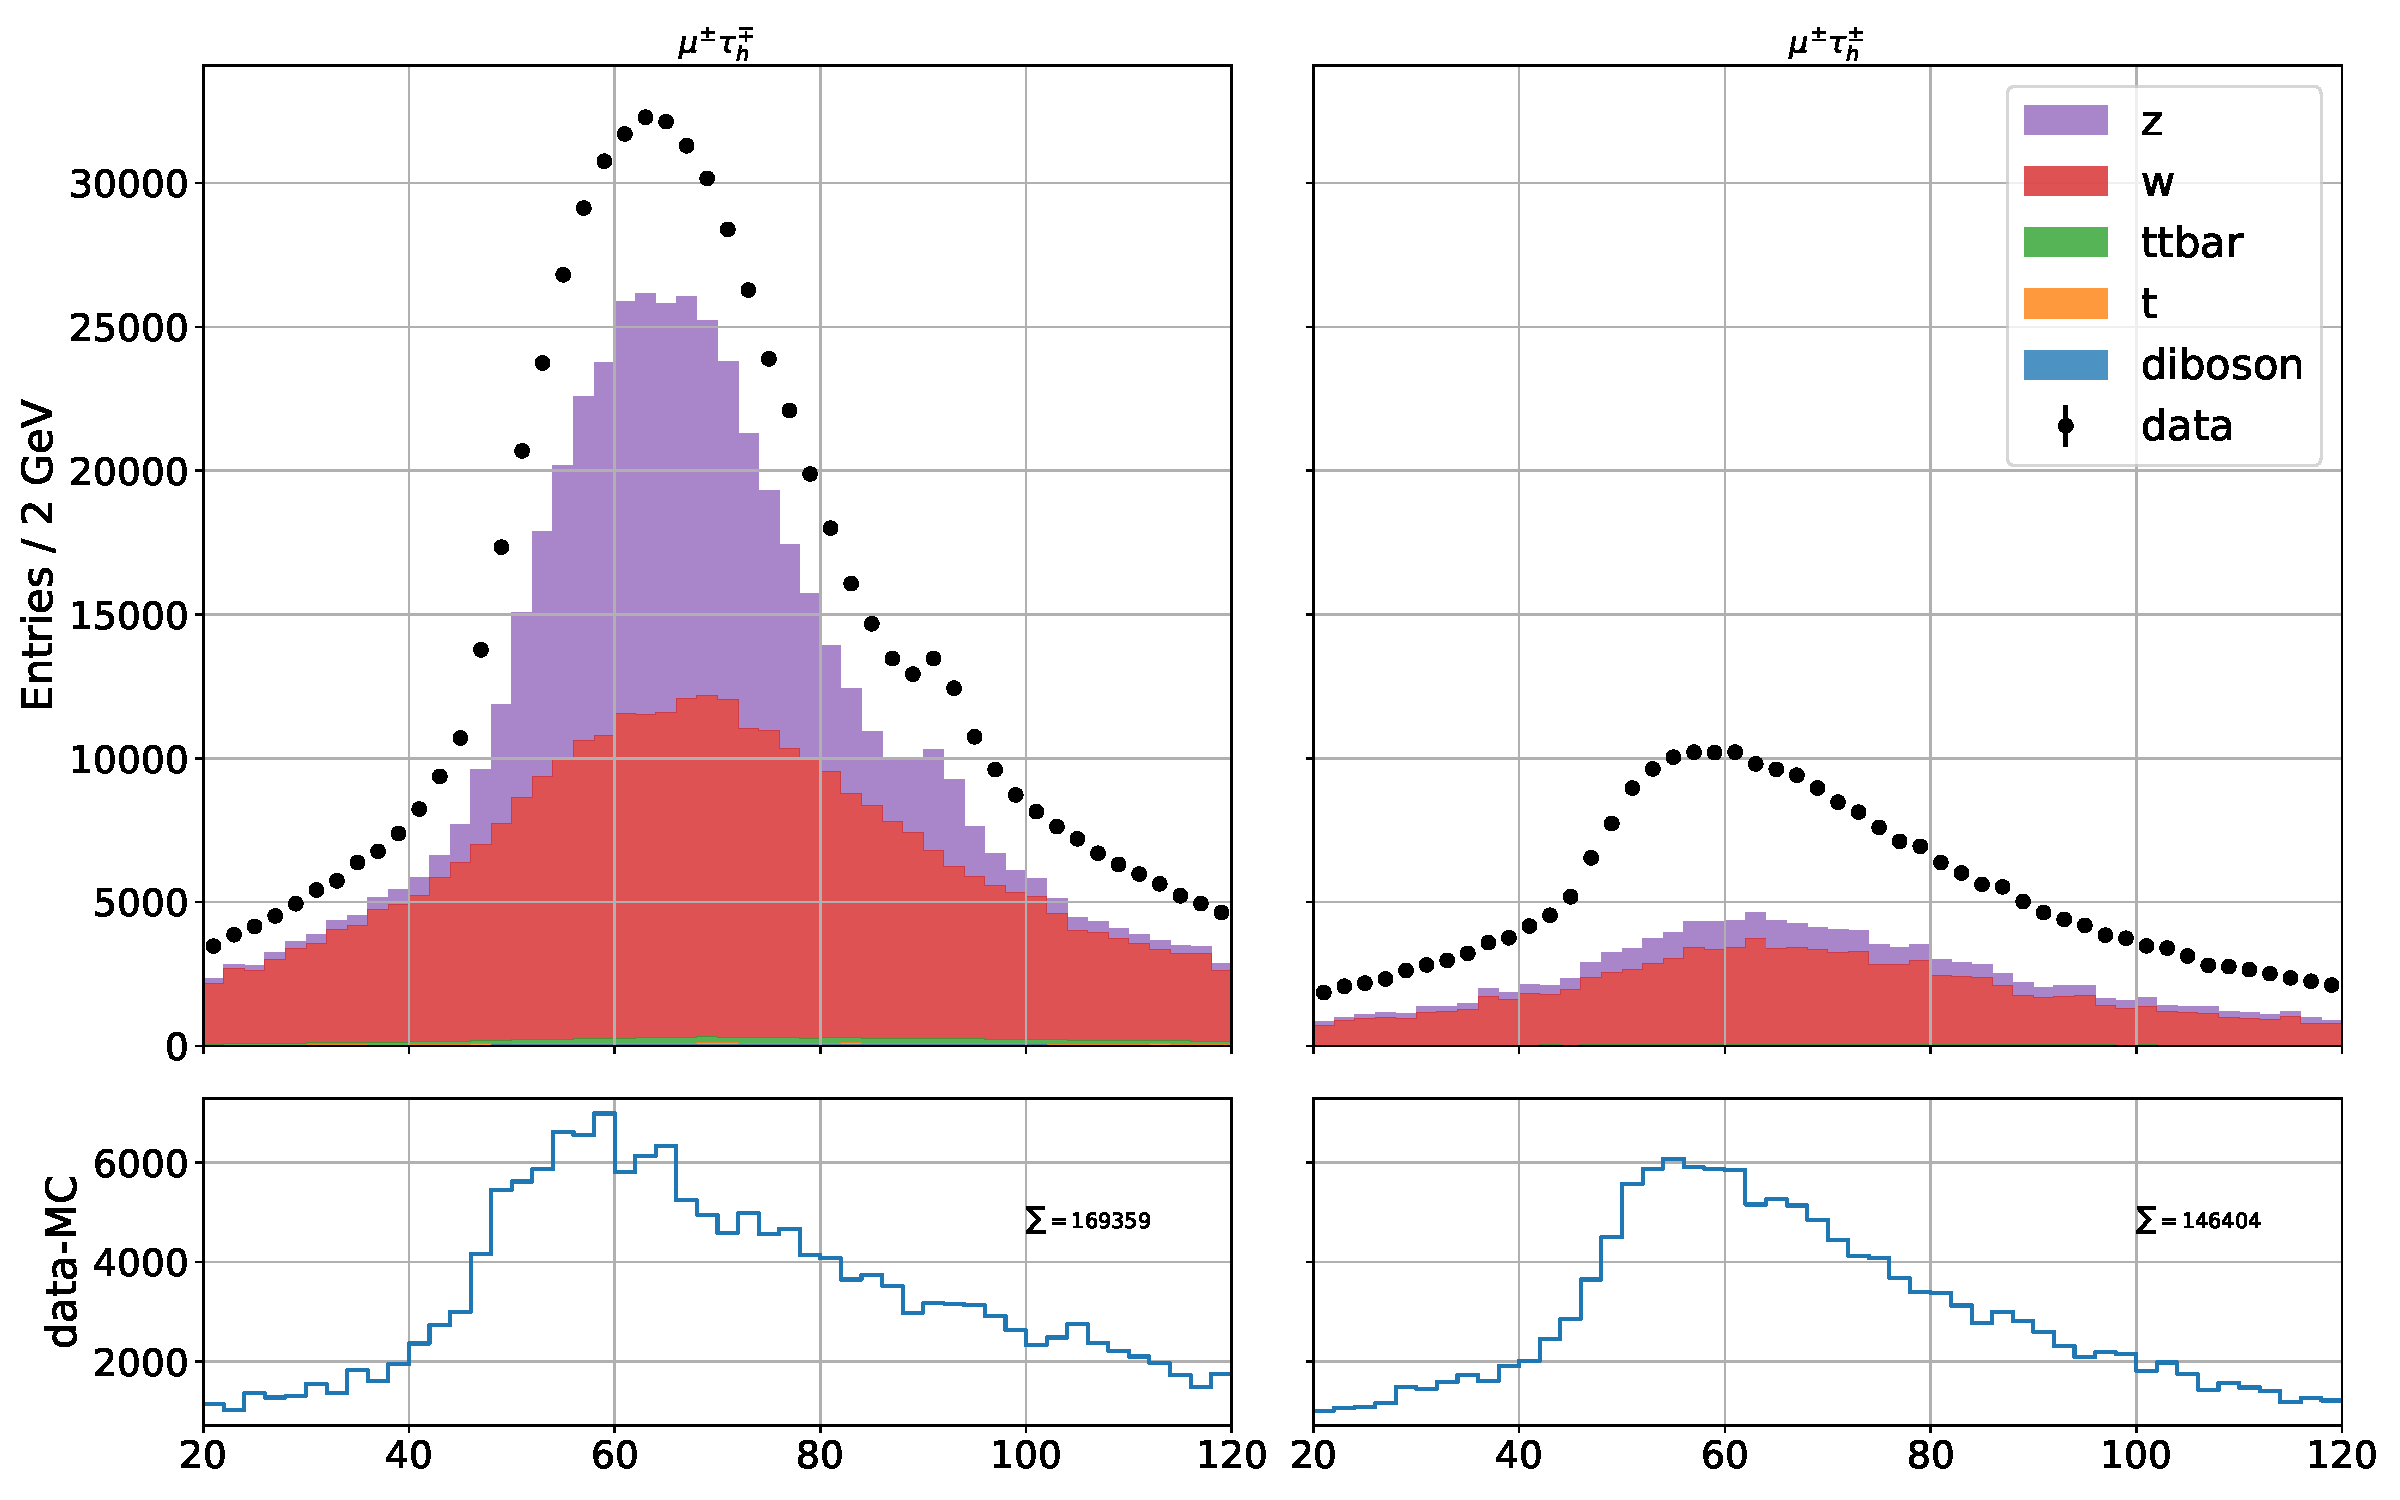
\includegraphics[width=0.9\textwidth]{chapters/Analysis/sectionBackground/figures/mutau_cr.pdf}
    \caption{Opposite sign (left) and same sign (right) control regions for the Z enriched $e\tau$ (top) and $\mu\tau$ (bottom) selection.}
    \label{fig:ltau_fakes}
\end{figure}


